\section{Methodology} \label{sec:methodology}
The primary goal to reach when analyzing dune field images is to compute and extract meaningful features, as discussed in \cite{ewing-kocurek-lake-2006,ewing-peyret-kocurek-bourke-2010}. The two main features extracted are the \emph{orientation} (local and global) and the \emph{inter dune spacing} (average distance between crest-lines). There are many potential methods to extract such features, but in this research, a crucial first step is to detect crest-lines in the dune field. Crest-lines are the main prominent features in any dune fields. The are characterized by a distinguishable peaks along a ridge of dunes. The need for automated detection of such features is very apparent. However, there are regions where dune fields are complex and dense, making automated dune detection a much more difficult task.

Generally, a crest-line is visible by the fact that it has a sunlit side, and a shaded side. Areas in the image where a bright region meets with a darker region are typically good candidates for potential crest-lines. This important criteria assumes that the sun's orientation is roughly perpendicular to the dune ridges. When ridges approach a parallel orientation to the sun's orientation, the crest-lines become less pronounced. One assumption is that crest-lines produce relatively stronger edges than other areas of the image. This assumption was the principle guiding criteria in \cite{2015_automated_mapping_of_linear_dunefield}. However, the strength of the edge depends on many factors. The sharpness of the actual dune ridge; sharper crest-lines will undoubtedly produce stronger, more defined edges on the satellite images. The sun's orientation and time of day also plays a role. As the sun approaches the horizon, the sunlit and shaded sides of the dunes become more defined. Inversely, when the sun is higher in the sky, shadows become less pronounced. Also, as discussed previously, the orientation relative to the dune field itself affects the strength of the edges. Finaly, scale, noise and resolution of the image can all affect the strength of edges.

Understanding the issues with the gradients of the key problem of this research. As shown in Figure \ref{fig:patches}, the pixel values and gradient magnitudes (edge strength) can vary greatly in each region. One inclination is to select strong gradients in an image as candidates for crest-lines (as done in \cite{2015_automated_mapping_of_linear_dunefield}). However, the gradients of crest-lines are not always larger than the gradients of valleys or the shadows. In Figure \ref{fig:patches}, a plot of the intensity, gradient magnitudes, and gradient orientations along a cross section of a crest-line is shown. In \cite{2015_automated_mapping_of_linear_dunefield}, the assumption was made that the weaker of the two edges can be filtered out, claiming that the larger peak is the crest-line, which is valid in the Kalahari image patch in Figure \ref{fig:kalahari_patch_plot}. However, the gradients produced by crest-lines may or may not be larger than their cast shadows, or the valleys. A clear example is shown in Figure \ref{fig:skeletoncoast_patch_plot}. Determining which peak to use can be accomplished using the gradient orientation, which is computed using the dominant orientation.

\begin{figure*}[htbp]
	\centering
	\begin{subfigure}[b]{0.1\textwidth}
		\centering
		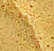
\includegraphics[width=\textwidth]{figures/kalahari_patch}
		\caption{}
		\label{fig:kalahari_patch}
	\end{subfigure}
	\begin{subfigure}[b]{0.1\textwidth}
		\centering
		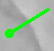
\includegraphics[width=\textwidth]{figures/kalahari_patch_arrow}
		\caption{}
		\label{fig:kalahari_patch_arrow}
	\end{subfigure}
	\begin{subfigure}[b]{0.6\textwidth}
		\centering
		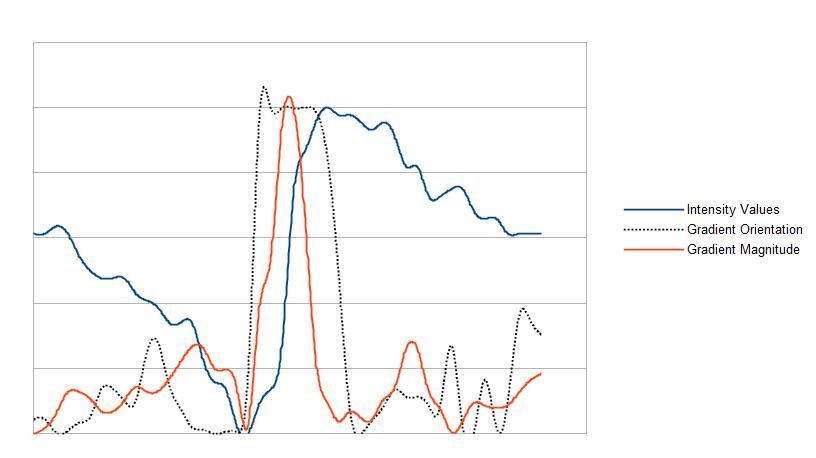
\includegraphics[width=\textwidth]{figures/kalahari_patch_plot}
		\caption{}
		\label{fig:kalahari_patch_plot}
	\end{subfigure}
	
	\begin{subfigure}[b]{0.1\textwidth}
		\centering
		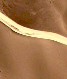
\includegraphics[width=\linewidth]{figures/skeletoncoast_patch}
		\caption{}
		\label{fig:skeletoncoast_patch}
	\end{subfigure}
	\begin{subfigure}[b]{0.1\textwidth}
		\centering
		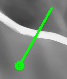
\includegraphics[width=\linewidth]{figures/skeletoncoast_patch_arrow}
		\caption{}
		\label{fig:skeletoncoast_patch_arrow}
	\end{subfigure}
	\begin{subfigure}[b]{0.6\textwidth}
		\centering
		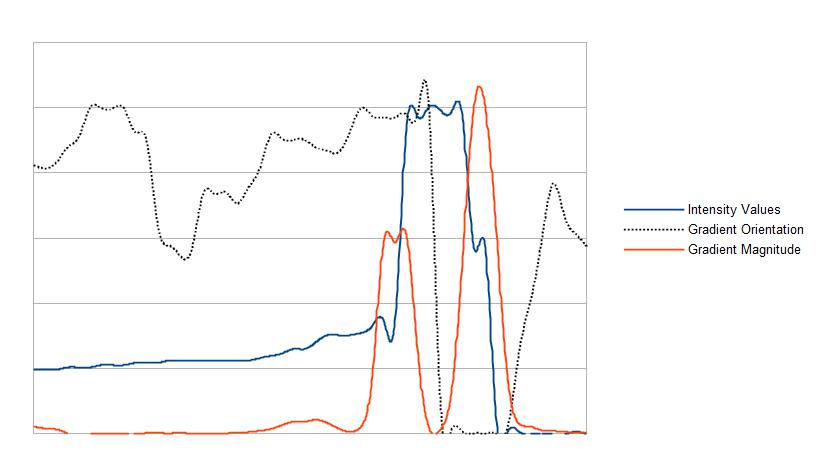
\includegraphics[width=\linewidth]{figures/skeletoncoast_patch_plot}
		\caption{}
		\label{fig:skeletoncoast_patch_plot}
	\end{subfigure}
	
	\caption{Illustration of the intensity, gradient magnitudes, and gradient orientations, plotted along a path crossing a dune crest-line: (\subref{fig:kalahari_patch}), (\subref{fig:skeletoncoast_patch}) a sample image patch from Kalahari and Skeleton Coast, (\subref{fig:kalahari_patch_arrow}) and (\subref{fig:skeletoncoast_patch_arrow}) the direction of the pixel samples plotted in (\subref{fig:kalahari_patch_plot}) and (\subref{fig:skeletoncoast_patch_plot}) containing the intensity, gradient magnitude and orientations values along the sampled direction. }
	\label{fig:patches}
\end{figure*}

\subsection{Process}

The processing stage is an important step to normalize and de-noise the input data. Images should have roughly the same scale. To enforce scale normalization, the data sets scales were manually selected for appropriate crest-line detection application, and the image resolutions were resized to similar sizes pixel in width. In future work, the dominant scale of the crest-lines could be determined automatically to improve the robustness of the algorithms. Images are also converted to gray scale, which improves processing performance and reduces the variability of illumination between different data sets. The final pre-processing step is to remove noise in the image using a low-pass filter. Many of the algorithms in this method rely on gradient information. Therefore, to extract the meaningful gradients, removing the highest frequencies (which in typically are responsible for noise), while preserving the lower scale or more desirable gradients. Two main popular filters are utilized. The median filter, introduced in \cite{huang_median_filtering_algorithm}, is applied first to remove grain and salt and pepper noise while preserving important edges. In some cases, median filtering also helps remove some smaller scale objects such as bushes, trees, rocks, and other features which are indistinguishable from satellite images. Following this, the standard Gaussian filter is applied which removes the remaining high frequency noisy signals from the image.

\subsection{Dominant Orientation} \label{subsec:dominant_orientation}
The dominant orientation is defined as the orientation of the gradients of crest-lines for the entire dune field. In datasets where the sun's azimuth is known, the dominant orientation can be directly calculated using the sun's orientation. However, in cases where this information is not provided, the dominant orientation must be computed automatically. Computing the dominant orientation of the dune field is an important step in the process. The dominant orientation is the overall gradient direction of the crest-lines to be detected. This process can help determine the average orientation of the dune field as well.

The direction of the gradient should agree with the overall dominant orientation of the dune field. Dunes typically have two major orientations, which are opposite directions. This phenomenon is clearly illustrated in Figure \ref{fig:patches}. Histograms of gradient directions can be used to determine the true orientation. Histograms have been used for many applications including \cite{lowe_sift_paper, dalal_histogram_oriented_gradients_human_detection, hu_gradient_field_descriptor}. Quantizing the space allows us to split edges according to their orientation, where each bin in the histogram represents an edge orientation. Each bin then covers an angle of $\frac{2\pi}{N}$radians, where \emph{N} is the number of bins. Each bin of the histogram is weighed by the magnitude of edges. Once the histogram is constructed, peaks in the magnitude will help determine the dominant orientation ($\varPhi$) of the dune crest-lines. In practice, a larger value for \emph{N} has shown to provide finer grain resolution which improves dominant orientation determination. 

As noted in \cite{2015_automated_mapping_of_linear_dunefield}, the histograms typically have a strong bimodal distribution. In some cases, the dominant peak of the histogram is not the part of the crest-line edge group, and the weaker one is. In that situation, choosing the higher peak will cause invalid crest-lines to be chosen. Histogram normalization can be applied to determine which peak best represents the crest-line edge group. The normalization process begins by computing the mean vector of the gradients from the edge image as follows:

\begin{equation}
\hat{\mu}\left\langle \bar{x},\bar{y}\right\rangle =\left\langle \frac{\sum_{i=0}^{P}\delta_{x_{i}}}{P},\frac{\sum_{i=0}^{P}\delta_{y_{i}}}{P}\right\rangle 
\end{equation}

where \emph{P} is the total number of detected edges from the Canny edge detector, $\delta_{x_{i}}$ and $\delta_{y_{i}}$ are the \emph{x} and \emph{y} gradient component of the \emph{i}\textsuperscript{th} point. The mean orientation is computed from the mean vector as:

\begin{equation}
\bar{\theta_{\mu}}=\arctan\left(\frac{\mu_{\bar{y}}}{\mu_{\bar{x}}}\right)
\end{equation}

The gradients are then normalized by simply subtracting the mean vector from each gradient:

\begin{equation}
\dot{\delta}\left(x_{i},y_{i}\right)=\left(\delta_{x_{i}}-\mu_{\bar{x}},\delta_{y_{i}}-\mu_{\bar{y}}\right)
\end{equation}

The normalized orientation $\dot{\theta_{i}}$ can be computed:

\begin{equation}
\dot{\theta_{i}}=\arctan\left(\frac{\dot{\delta_{y_{i}}}}{\dot{\delta_{x_{i}}}}\right)
\end{equation}

To determine which bin the \emph{i}\textsuperscript{th} edge point belongs to, we simply calculate $\left\lceil \frac{\dot{\theta_{i}}\centerdot N}{2\pi}-0.5\right\rceil $,	and increment that bin by the magnitude of the normalized gradient	by $\sqrt{\dot{\delta}_{x_{i}}^{2}+\dot{\delta}_{y_{i}}^{2}}$. In essence, this normalization process removes the uneven skew of the gradients in the overall image. Removing this skew allows true crest-line edges to be fairly compared with other stronger edges. The normalization process softens the stronger dominant edge which enables true crest-lines to be accurately determined in images where the valleys of dunes are sharp and contain strong edges.

Once the histogram is computed and normalized, the dominant orientation vector $\hat{\theta_{dom}}$ is determined by averaging the gradients belonging to the histogram bin with the highest value. With the dominant orientation knowledge acquired, candidate crest-line dunes can be detected. The dominant orientation will always point from the shaded area of the dune towards the sunlit area. This phenomenon is due to the gradient operator. Subtracting a dark pixel (lower value) from a bright pixel (larger value), results in a positive value, which in terms means that the gradients of darker pixels always point towards brighter pixels. Given this fact, a case can be made for comparing the gradients of each pixel to the dominant orientation vector. All gradient vectors which \emph{agree} with the dominant orientation are then considered to be the shaded sides of a dune, and all gradients which \emph{disagree} with the dominant orientation are therefore part of the sunlit side of a dune. Finally the transition between areas that \emph{agree} and those that \emph{disagree} must be a good potential crest-line candidate.

The concept of \emph{agreement} can be defined mathematically using a simple dot product. Given an dominant orientation defined as a unit length vector $\hat{\delta_{\mu}}$, and the local unit length gradient vector at (i, j) defined as

\begin{equation}
\hat{\delta_{ij}} = \left\langle \frac{\delta_{x_{ij}}}{\sqrt{\delta_{x_{ij}}^2 + \delta_{y_{ij}}^2}}, \frac{\delta_{y_{ij}}}{\sqrt{\delta_{x_{ij}}^2 + \delta_{y_{ij}}^2}}\right\rangle 
\end{equation}

The \emph{agreement} measurement $D_{ij}$ then is simply the dot product:

\begin{equation}
D_{ij} = \hat{\delta_{ij}} \bullet \hat{\delta_{\mu}}
\end{equation}

Since $\hat{\delta_{ij}}$ and $\hat{\delta_{\mu}}$ are both unit-length vectors, the range possible values for $D_{ij}$ is $[-1, 1]$, where positive values represent gradients which \emph{agree} with the dominant orientation, 0 is perpendicular to the dominant orientation, and negative values \emph{disagree} with the dominant orientation. The result of the dot product computed at each pixel is shown in Figure \ref{fig:orientation_based_dot_product}, which we call the gradient direction map.

The regions produced by the gradient direction map have been shown to be typically smooth and have good continuity in this application. There appears to be a clear separation between regions in \emph{agreement} and other regions. The separation becomes even clearer when the gradient direction map is thresholded based on the dot product values. In Figure \ref{fig:orientation_based_threshold_dot_product}, a binary image of the gradient direction map is computed by thresholding all dot products above 0. Once the gradient direction map has been thresholded, the binary image provides well defined regions which allows the use of contours to determine the crest-lines. The contours extracted provide good continuity of the crest-lines, but also contain many elements which are not part of the crest-line. A drawback of the gradient orientation map is the inherent localization problem due to the computation of the gradient orientation and size of the kernel to compute the gradients. The contours detected will inevitably land on the orientation transition and will almost always be shifted slightly away from the true crest-line. In order to improve localization, the contours must be shifted towards to nearest likely crest-line candidate. Each point on the contour can then be shifted by the computed distance to each crest-line candidate.


\subsection{Detecting Crest-Line Candidates}

The detection step seeks to extract candidate segments which are most likely candidates for crest-lines. Candidates for crest-lines can be found using machine learning methods which can learn the features specific to crest-lines versus non-crest-lines, thus the filtering can be accomplished using a trained model. A similar approach was implemented in \cite{2006_automated_classification_landform_elements,2007_Machine_Learning_tools_automatic_mapping_mars,2013_sar_image_automated_detection_dune_area,BandeiraMarques,2011_neural_network_based_dunal_landform_mapping,vaz_object_based_dune_analysis}. The goal is to train a machine learning model using a training data set, then generate the response map which is the response of the model at each pixel in a given image. Ideally, the responses are high at pixels which contain crest-lines, and low everywhere else. To improve the localization, the contours are shifted towards the nearest peak in the response map.

Machine learning techniques typically require training data to construct the model in order to reliably solve classification problems. This method of training is called supervised learning (\cite{foundations_machine_learning_book,machine_learning_book}). For crest-line detection, we therefore need to split our data into two classes: crest-lines and non-crest-lines. In this application, our data sets included the ground truth for each image set. The ground truth is essentially a binary image with the labeled crest-lines. From the set of training images, the ground truth images are used to extract locations of crest-lines and non-crest-lines. For each image, pixel positions are chosen randomly, if the ground truth at the position contains a crest-line, the pixel location is added to the crest-line set, otherwise it is added to the non-crest-line set. The sampling is optimized so that \emph{N} samples are chosen for each class. The next step in the process flow is to extract features from each of these samples, which will be used to feed into the model for training and validation.

Features or descriptors are typically vectors of values which describes the local neighborhood around a pixel location (\cite{lowe_sift_paper,1994_good_features_to_track,1998_feature_detection,2007_invariant_features_survey}). Descriptors can range from simple pixel values in an image patch, to gradient information, to more sophisticated descriptors such as HOG (Histogram of Oriented Gradients \cite{2007_hog_human_detection}), LBP (Local Binary Pattern \cite{1994_lbp_paper,1996_lbp_paper}), Haar Features (\cite{2001_viola_jones_paper}), SURF (Speeded Up Robust Features \cite{2006_surf}), SIFT (Scale Invariant Feature Transform \cite{lowe_sift_paper}), and many more. 

The SIFT descriptor has been shown to provide the best overall results. The SIFT descriptor is computed over a fixed-size window around every pixel, with the orientation calculated using the gradients at the local pixel location. In future work, there could be some improvements to results by computing the local scale and computing the orientation at the computed scale. After computing the descriptor for each crest-line and non-crest-line training/validation samples, the classifier model can then be trained, optimized, and validated. There are many different kinds of classifiers in machine learning: Bayesian, decision trees, artificial neural networks, Support Vector Machines, and many more (\cite{book_artificial_intelligence_modern_approach,2003_tackling_poor_assumptions_naive_bayes,1987_simplifying_decision_trees,1943_logical_calculus_ideas_immanent_nervous_activity,book_organization_of_behavior,1975_beyond_regression_prediction_analysis,1995_support_vector_networks,1995_support_vector_clustering}). As part of this research, we studied the various classifiers, notably SVM and Gradient Boosted Trees (\cite{1999_gradient_boosting_machine,1999_stochastic_gradient_boosting}) which provided the best performance with the SIFT features for crest-line recognition. Once trained, the models are capable of recognizing pixels which contain crest-lines.

The next step is to construct a response map at each pixel of the images. Since the classifier was trained to output 1 (for crest-lines) or -1 (for non-crest-lines), the range of response values is then $[-1, 1]$. The resulting image is the response map of candidate crest-line. The response map therefore produces an image where bright regions are likely crest-line candidates. Gradient Boosted Trees classifiers seems to produce the best results. The results of the Gradient Boosted Trees classifier training are shown in Table \ref{tab:boosted_trees_training_test_results}. In Figure \ref{fig:kalahari_response}, an example of a response map produced by the GBT classifier on the Kalahari image is shown.

The final step is to improve the localization of the crest-lines using the response map, by translating the detected contours towards the nearest peaks in the response map. The shift can be determined by doing a search along the opposite direction of the dominant orientation. Smoothing can be applied in order to ensure that segments remain contiguous after the translation is applied. Once the shift has been applied to every contour segments, filtering non-crest-line segments can be done by simply removing all contour segments which fall on weak responses. After all contours have been filtered, the remaining segments can be further filtered by segment length. All segments which are too short are removed from candidate crest-line segments. The overall output of this process is shown in Figure \ref{fig:kalahari_results}. Once all crest-line candidates have been detected, the dune field's morphological properties can be computed.


\begin{figure*}[htbp]
	\centering
	\begin{subfigure}[b]{0.3\textwidth}
		\centering
		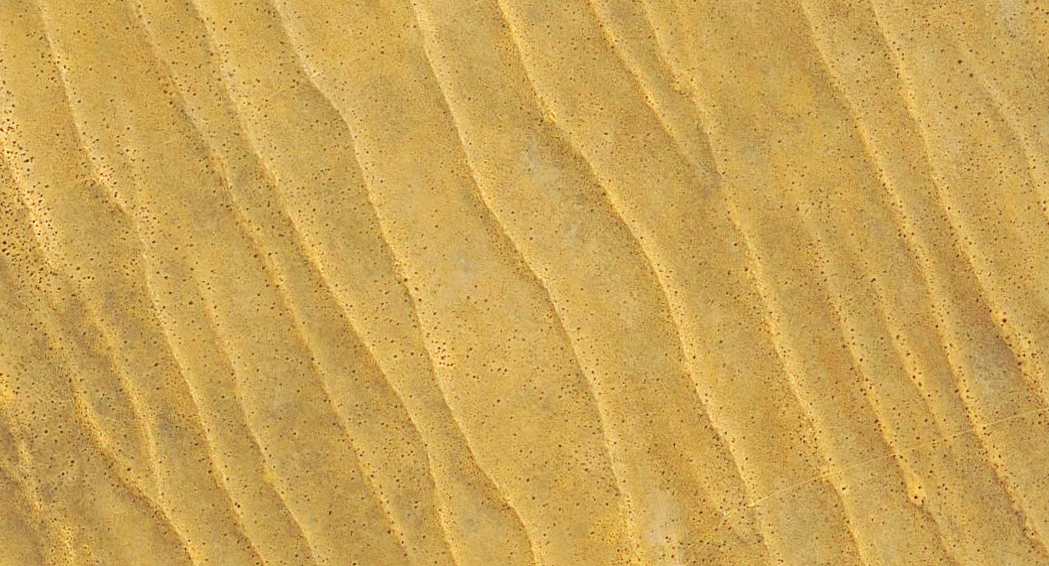
\includegraphics[width=\linewidth]{figures/kalahari}
		\caption{Kalahari}
		\label{fig:orientation_based_kalahari}
	\end{subfigure}
	\begin{subfigure}[b]{0.3\textwidth}
		\centering
		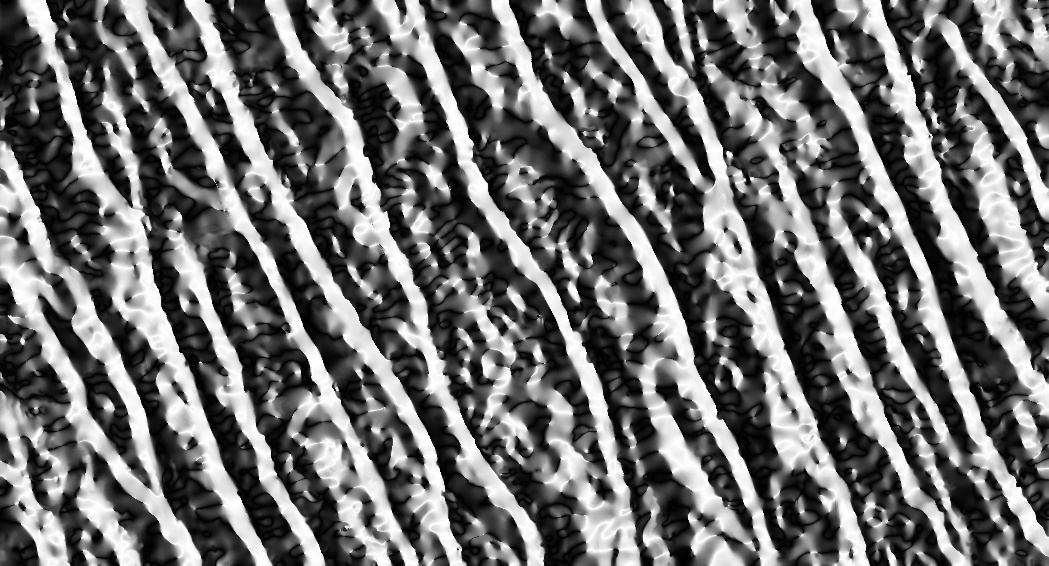
\includegraphics[width=\linewidth]{figures/gradient_direction_image}
		\caption{Gradient direction map \emph{D}}
		\label{fig:orientation_based_dot_product}
	\end{subfigure}
	\begin{subfigure}[b]{0.3\textwidth}
		\centering
		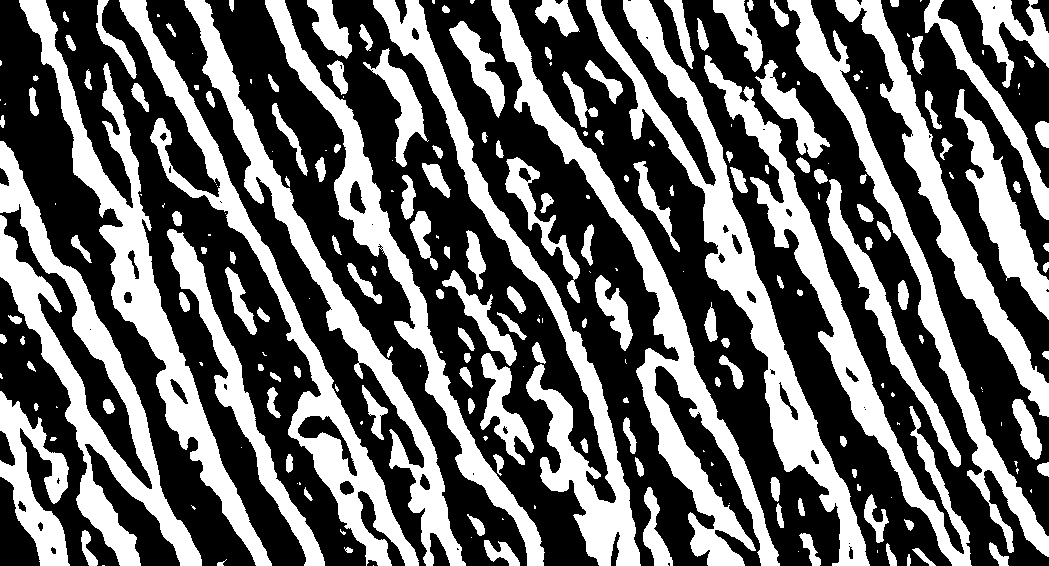
\includegraphics[width=\linewidth]{figures/gradient_direction_thresholded_image}
		\caption{$D_{ij} > 0$}
		\label{fig:orientation_based_threshold_dot_product}
	\end{subfigure}
	\begin{subfigure}[b]{0.45\textwidth}
		\centering
		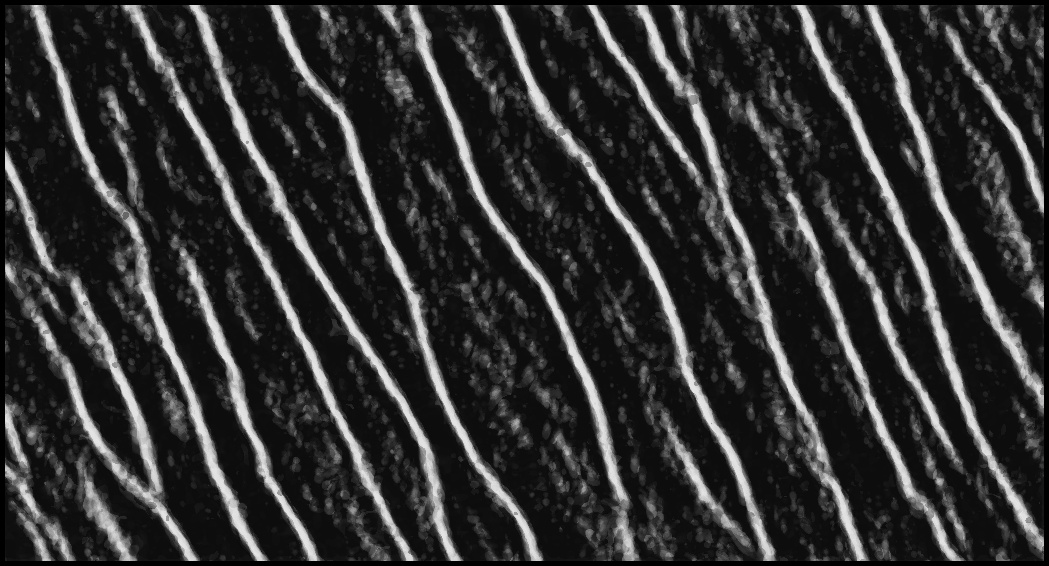
\includegraphics[width=\linewidth]{figures/kalahari_response}
		\caption{Response Map (GBT)}
		\label{fig:kalahari_response}
	\end{subfigure}
	\begin{subfigure}[b]{0.45\textwidth}
		\centering
		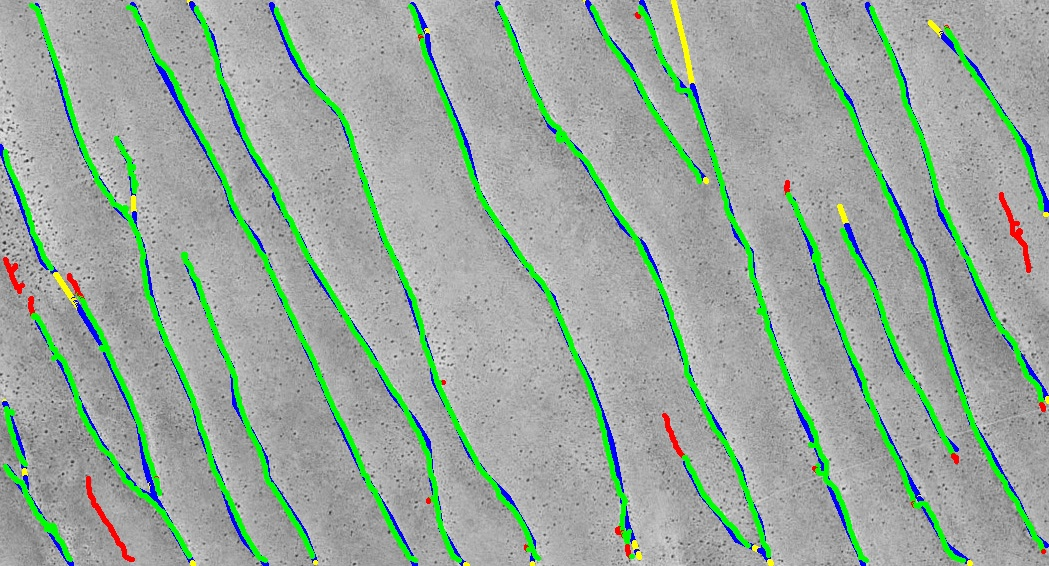
\includegraphics[width=\linewidth]{figures/kalahari_results}
		\caption{Crest-line Detection}
		\label{fig:kalahari_results}
	\end{subfigure}
	\caption{The approach illustrated: (\subref{fig:orientation_based_kalahari}) The input image from the Kalahari, (\subref{fig:orientation_based_dot_product}) The gradient direction map \emph{D} computed by taking the dot product of the gradients at each pixel with the dominant orientation, (\subref{fig:orientation_based_threshold_dot_product}) thresholding the gradient direction map for all dot products greater than 0, (\subref{fig:kalahari_response}) the response map computed using Gradient-Boosted Trees, (\subref{fig:kalahari_results}) the results of crest-line detection after contour shifting and filtering, where green lines are true positives, red lines are false positives. yellow is false negative, and blue is the ground truth. }
	\label{fig:orientation_based_process}
\end{figure*}


\subsection{Dune Metrics Calculations} \label{subsec:dune-field-metrics}
The final step of the process is to extract meaningful features and metrics for researchers to study from the dune fields. This process requires a good set of detected crest-lines. The output crest-line segments extracted in the previous methods are used as input for computing the features. There are many features metrics of interests to scientists in this field, including dune spacings, orientation, shape, size, length, bifurcations, and many more. These metrics can be used to study and understand the movements of various patterns of dunes over time in a specific area.

As part of this research, we focused mainly on orientation and spacing of dunes, and used those metrics as validations for the effectiveness of the dune detection methods. Although these metrics are not a complete evaluation of the dune field, they are sufficiently complex to provide valuable feedback for scientists. In order to compute the average dune field orientation from the detected points, the data must be formatted appropriately. The detected crest-lines are typically a set of two dimensional points on the image. These points form lines and segments of various shapes and lengths. The simplest way to compute the orientation is to fit lines to each segments and compute the average orientation of the lines. There are many commonly used methods to fit lines to segments. One popular method is the Hough Transform initially proposed in \cite{hough-1959-paper,hough-1962-patent,hough-duda-1972-paper}, which searches a space of parameters voting for segments which contribute to the line. The Hough transform can be generalized to many shapes suchs as circles and ellipses, but the parameter space gets much larger for complex shapes. The main drawback of the Hough transform is the computational cost of search a large parameter space.

An alternative method is the Ramer-Douglas-Peucker algorithm, proposed in \cite{ramer-1972-paper,douglas-peucker-1973-paper,douglas-hershberger-snoeyink-1992-paper}, with the implementation provided within the OpenCV (\cite{opencv_library}) framework. The method is used for simplifying or approximating any given curve to a subset of points. Thus, the dune segments can be reduced to subset of lines. The only parameter required is the allowable error in the approximation. Larger values allow more deviation, producing longer coarse approximations of the segments, while smaller values approximate the curve more closely, producing short segments which are sensitive to noise. The parameter is chosen to produce optimal results for the application. As explained in \cite{computing-average-orientation-of-vectors}, computing the average orientation of vectors is not as trivial as simply averaging the orientations. To illustrate the problem, the average of an angle of $350^{\circ}$ and $10^{\circ}$ would be $180^{\circ}$, when in fact a more appropriate average should be $0^{\circ}$. Averaging may produce an adequate approximation, but the von Mises distribution based method proposed in \cite{computing-average-orientation-of-vectors} typically produces much more accurate results. Therefore, this technique is used to compute the average orientation of the lines.

With the orientation of the dune field computed, the average dune distance can then be computed. Computing the distance between crest-lines is a feature interesting to many researchers in the field. For simplicity, the inter-dune spacing is computed for the entire dune field image. The resulting measurement is in pixels in our case, but, if the scale of the satellite image is known (meters per pixels), then the measurement can be easily converted to a real world measurement. Using the binary image of the extracted dune crest-lines, and the average orientation computed, an iterative approach is used to measure the distance between the dunes. A search is done at each pixel along an orthogonal axis from the average orientation. When a crest-line is hit, the number of pixels traveled are counted until another dune is found. The process is repeated for the entire binary image. The lengths are averaged resulting in the average dune spacing for the entire dune field. The results produced may not be optimal and accurate but can be used as an indicator to evaluate the effectiveness of the dune crest-line detection. The results and metrics are presented in section \ref{subsec:results-and-discussion}.
